\newpage
%Color
\definecolor{ChetwodeBlue}{rgb}{0.556,0.662,0.858}

\section{CAPITULO IV}
\section*{PROPUESTA TÉCNICA DE LA MEJORA}
En este capítulo, se propone una solución técnica para abordar las deficiencias identificadas, con un enfoque en la mejora de los procesos operativos. Se presentan aspectos como la metodología de implementación, recursos técnicos necesarios, cronograma de ejecución y posibles limitaciones que podrían surgir durante el proceso de implementación. A través de la planificación detallada y la asignación de responsabilidades claras, se busca garantizar que la implementación de las mejoras se realice de manera eficiente y efectiva, maximizando los beneficios para la empresa.


\subsection{4.1 Plan de acción de la Mejora propuesta}
%El plan de acción es una herramienta importante en el proceso de implementación de mejoras. Este plan detalla las diversas tareas y actividades necesarias para llevar a cabo la mejora, asignando responsabilidades, recursos y tiempos para cada una de ellas. Esta representado en la tabla 4, constituye un plan que prioriza las iniciativas más importantes para cumplir con los objetivos y/o metas del proyecto. De esta manera, se podrá constituir un plan de acción que nos servirá de guía a la hora de llevar el mismo.

El plan de acción es una herramienta importante en el proceso de implementación de mejoras. Este plan detalla las diversas tareas y actividades necesarias para llevar a cabo la mejora, asignando responsabilidades, recursos y tiempos para cada una de ellas. Representado en la tabla 4, constituye un plan que prioriza las iniciativas más importantes para cumplir con los objetivos y/o metas del proyecto. De esta manera, se podrá constituir un plan de acción que servirá de guía a la hora de llevarlo a cabo.

La tabla 4 proporciona un desglose detallado de las tareas necesarias para implementar una mejora en un sistema de software. Incluye actividades clave como la identificación de requisitos, el diseño y desarrollo de interfaces, la implementación de la arquitectura backend y la integración del frontend y backend. Cada tarea está asignada a un responsable específico y se detallan los recursos necesarios, el tiempo estimado de cada actividad y los indicadores de seguimiento para monitorear el progreso. El plan asegura que cada etapa del proyecto esté bien definida y organizada para facilitar una implementación eficiente y sin problemas en un entorno de producción.

%Diagrama plan de mejora
\begin{landscape}
\begin{table}
\centering
\caption{Plan de acciones de la mejora}
\begin{tblr}{
  cells = {c},
  row{1} = {ChetwodeBlue},
  column{1} = {3.5cm},
  column{2} = {5cm},
  column{3} = {2.2cm},
  column{4} = {0.4cm},
  column{5} = {3cm},
  column{6} = {3.5cm},
  column{7} = {2.8cm},
  cell{2}{3} = {r=2}{},
  cell{2}{7} = {r=9}{},
  cell{7}{3} = {r=2}{},
  cell{7}{5} = {r=3}{},
  vlines,
  hline{1-2,11} = {-}{},
  hline{3} = {1-2,4-6}{},
  hline{4-7,10} = {1-6}{},
  hline{8} = {1-2,4,6}{},
  hline{9} = {1-4,6}{},
}
\textbf{Acciones de Mejora} & \textbf{Tareas} & \textbf{Responsable} & \textbf{T (h)} & \textbf{Recursos Necesarios} & \textbf{Indicador de Seguimiento} & \textbf{Responsable de Seguimiento}\\
Listar requisitos del sistema & Reunión con usuarios para identificar requisitos & Analista de Sistemas & 16 & Hojas & Requisitos & Monitor de empresa\\
Análisis de requisitos & Elaboración de documentación técnica y diagramas &  & 16 & Herramientas de diseño de software & Documentación & \\
Diseño de la interfaz & Creación de prototipos de interfaz & Diseñador UX/UI & 32 & Herramientas de diseño de interfazces & Prototipos aprobados & \\
Desarrollo de la interfaz & Implementación de la interfaz de usuario & Programador & 40 & Entorno de desarrollo & Interfaz funcional. & \\
Diseño de la arquitectura Backend & Definición de la arquitectura usada en el Back-End & Analista de Sistemas & 16 & Herramientas de diseño de software & Arquitectura aprobada & \\
Implementación del Back-end & Codificación de los componentes del sistema & Programador & 64 & Entorno de desarrollo & Sistema Back-End funcional. & \\
Unión del Front-End y Back-End & Codificación de los servicios requeridos para unir ambos lados del sistema &  & 24 &  & Componentes unidos & \\
Pruebas de funciomiento & Verificar que todos los módulos funcionan sin errores & Tester & 24 &  & Módulos funcionando correctamente & \\
Implementación del sistema en entorno de producción & Configuración de servidores y bases de datos & Programador & 24 & Servidores, Bases de datos, AWS & Sistema funcionando correctamente & 
\end{tblr}
\end{table}

\end{landscape}

%\begin{landscape}
%\begin{table}
%\centering
%\captionsetup{labelformat=empty}
%\begin{tblr}{
%  row{1} = {ChetwodeBlue},
%  column{1} = {3.5cm},
%  column{2} = {5cm},
%  column{3} = {2.2cm},
%  column{4} = {0.4cm},
%  column{5} = {3cm},
%  column{6} = {3.5cm},
%  column{7} = {2.8cm},
%  cell{2}{5} = {r=2}{},
%  cell{2}{7} = {r=3}{},
%  vlines,
%  hline{1-2,5} = {-}{},
%  hline{3} = {1-4,6}{},
%  hline{4} = {1-6}{},
%}
%\textbf{Acciones de Mejora} & \textbf{Tareas} & \textbf{Responsable} & \textbf{T (h)} & \textbf{Recursos Necesarios} & \textbf{Indicador de Seguimiento} & \textbf{Responsable de Seguimiento}\\
%Unión del Front-End y Back-End & Codificación de los servicios requeridos para unir ambos lados del sistema & Programador & 24 & Entorno de desarrollo & Componentes unidos & Monitor de empresa\\
%Pruebas de funciomiento & Verificar que todos los módulos funcionan sin errores & Tester & 24 &  & Módulos funcionando correctamente & \\
%Implementación del sistema en entorno de producción & Configuración de servidores y bases de datos & Programador & 24 & Servidores, Bases de datos, AWS & Sistema funcionando correctamente & 
%\end{tblr}
%\end{table}


%\captionsetup{labelformat=empty}
%\begin{longtable}{|p{3.5cm}|p{5cm}|p{2.2cm}|p{0.4cm}|p{3cm}|p{3.5cm}|p{2.8cm}|}
%%\caption[Plan de acciones de la mejora]{\textbf{Plan de acciones de la mejora}}\\
%\hline
%\rowcolor[rgb]{0.557,0.663,0.859} \textbf{Acciones de Mejora} & \textbf{Tareas} & \textbf{Responsable} & \textbf{T (h)} & \textbf{Recursos Necesarios} & \textbf{Indicador de Seguimiento} & \textbf{Responsable de Seguimiento} \endfirsthead 
%\hline
%Unión del Front-End y Back-End & Codificación de los servicios requeridos para unir ambos lados del sistema & Programador & 24 & Entorno de desarrollo & Ambos sistemas unidos correctamente & Monitor de empresa \\ 
%\hline
%Pruebas de funciomiento & Verificar que todos los módulos funcionan sin errores & Tester & 24 & Entorno de desarrollo & Módulos del sistema funcionando correctamente & Monitor de empresa \\ 
%\hline
%Implementación del sistema en entorno de producción & Configuración de servidores y bases de datos & Programador & 24 & Servidores, Bases de datos, AWS & Sistema funcionando correctamente en un entorno de producción & Monitor de empresa \\
%\hline
%\end{longtable}
%\end{landscape}



\subsection{4.2 Consideraciones técnicas para la implementación de la mejora}
En esta sección se detallan los aspectos técnicos que han sido considerados para la implementación de la mejora en el sistema de gestión del taller mecánico. La implementación exitosa de un sistema de software no solo depende de un buen diseño y programación, sino también de la correcta planificación y consideración de diversos factores técnicos que aseguren un desempeño óptimo y una integración eficaz con la infraestructura existente. A continuación, se presentan las principales consideraciones técnicas, incluyendo las especificaciones del equipo, los diagramas de casos de uso, el diagrama de clases, y el diagrama de implementación, así como una lista de recursos técnicos necesarios para llevar a cabo la mejora propuesta.


\subsubsection*{4.2.1 Consideraciones técnicas.}
Para asegurar que el proceso de desarrollo se lleve a cabo de manera eficiente y efectiva, es crucial considerar las especificaciones técnicas del equipo utilizado. Estas especificaciones incluyen detalles sobre el hardware y software empleados por los desarrolladores, que son fundamentales para garantizar la compatibilidad y el rendimiento adecuado del sistema. En la Diagrama 6, se proporciona una ficha técnica que describe en detalle las características del equipo utilizado durante el desarrollo del sistema. Esta información es esencial para entender las capacidades y limitaciones técnicas con las que se ha trabajado y cómo estas influencian el proceso de desarrollo.

En esta sección, se presentan las consideraciones técnicas que fueron tomadas en cuenta durante la implementación de la mejora. Estas consideraciones incluyen las especificaciones del equipo utilizado por el desarrollador durante el proceso de desarrollo del sistema, estas características son descritas en el diagrama 6.

%Ficha tecnica
\begin{figure}[H]
    \caption{Ficha Técnica}
    \begin{tabular}{c}
        %\includesvg[width=1\textwidth]{imagenes/cap3/DOP1.svg} \\
        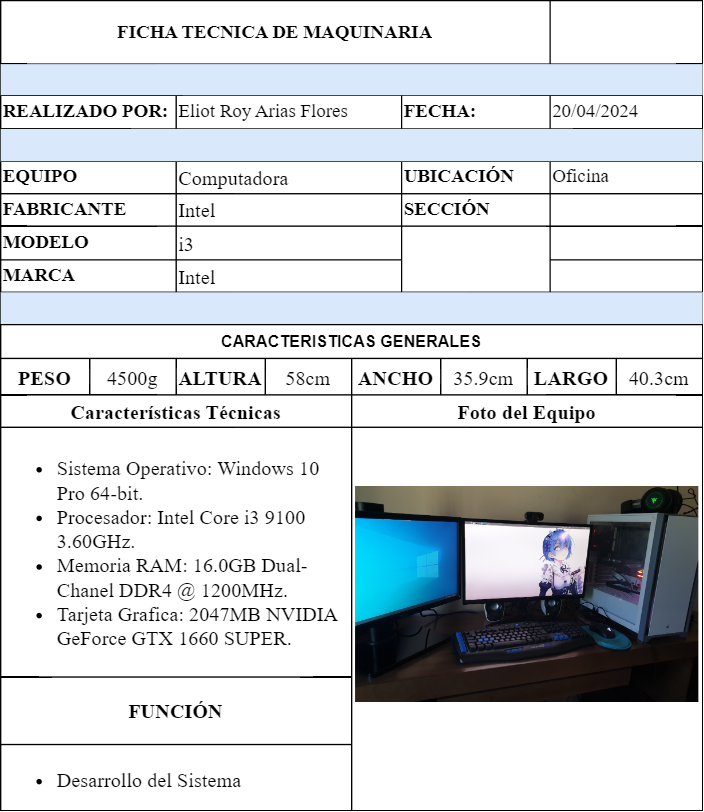
\includegraphics[width=16cm, height=17cm]{imagenes/cap4/FichaTecnica1.png}
    \end{tabular}
    \label{fig:fichaTecnica}
\end{figure}


\subsubsection*{4.2.2 Diagrama de casos de Uso}
El diagrama de casos de uso es una herramienta fundamental dentro de la metodología UML (Unified Modeling Language) que permite visualizar las interacciones entre los usuarios (en este caso, el administrador) y el sistema. Este diagrama ayuda a identificar y organizar las funcionalidades clave del sistema en paquetes específicos, cada uno de los cuales agrupa un conjunto de acciones relacionadas que el usuario puede realizar.

\begin{enumerate}
	\item Gestión de Clientes: Este paquete se encarga de las funcionalidades relacionadas con la gestión de clientes, incluyendo el registro, actualización, búsqueda y eliminación de clientes.
	\begin{itemize}
		\item \textbf{Gestionar Clientes:} Permite al administrador acceder a todas las funcionalidades relacionadas con los clientes.
		\item \textbf{Registrar Cliente:} Permite al administrador registrar un nuevo cliente en el sistema.
		\item \textbf{Actualizar Cliente:} Permite al administrador actualizar la información de un cliente existente en el sistema.
		\item \textbf{Buscar Cliente:} Permite al administrador buscar clientes en la base de datos según ciertos criterios.
		\item \textbf{Eliminar Cliente:} Permite al administrador eliminar un cliente del sistema.
		\item \textbf{Validar Datos:} Verifica que los datos ingresados o actualizados del cliente sean válidos y completos.
	\end{itemize}
	\begin{figure}[H]
		\centering
		\caption{Gestión de Clientes}
		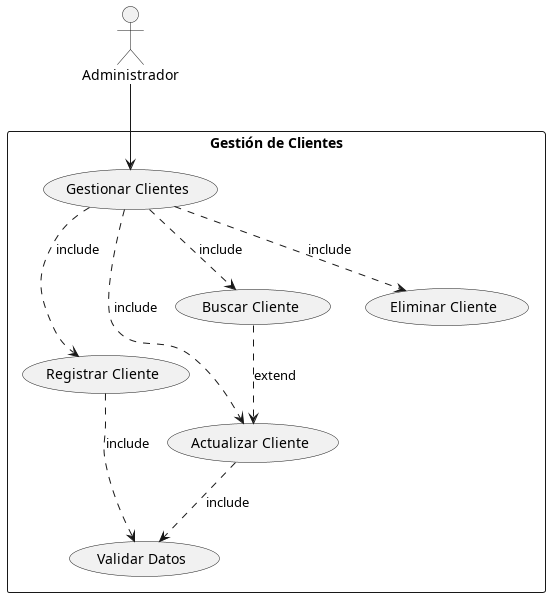
\includegraphics[width=12cm, height=8cm]{imagenes/cap4/casosUso/GestionClientes.png}
		\label{fig:Caso1}
	\end{figure}
	
	\item Gestión de Vehículos: Este paquete se enfoca en las funcionalidades relacionadas con la gestión de vehículos, incluyendo el registro, actualización, búsqueda y eliminación de vehículos.
	\begin{itemize}
		\item \textbf{Gestionar Vehículos:} Permite al administrador acceder a todas las funcionalidades relacionadas con los vehículos.
		\item \textbf{Registrar Vehículo:} Permite al administrador registrar un nuevo vehículo en el sistema.
		\item \textbf{Actualizar Vehículo:} Permite al administrador actualizar la información de un vehículo registrado en el sistema.
		\item \textbf{Buscar Vehículo:} Permite al administrador buscar vehículos en la base de datos según ciertos criterios.
		\item \textbf{Eliminar Vehículo:} Permite al administrador eliminar un vehículo del sistema.
		\item \textbf{Ver Detalles del Vehículo:} Permite al administrador obtener detalles específicos de un vehículo registrado en el sistema.
		\item \textbf{Asociar Vehículo a Cliente:} Permite al administrador vincular un vehículo con su propietario en el sistema.
	\end{itemize}
	\begin{figure}[H]
		\centering
		\caption{Gestión de Vehículos}
		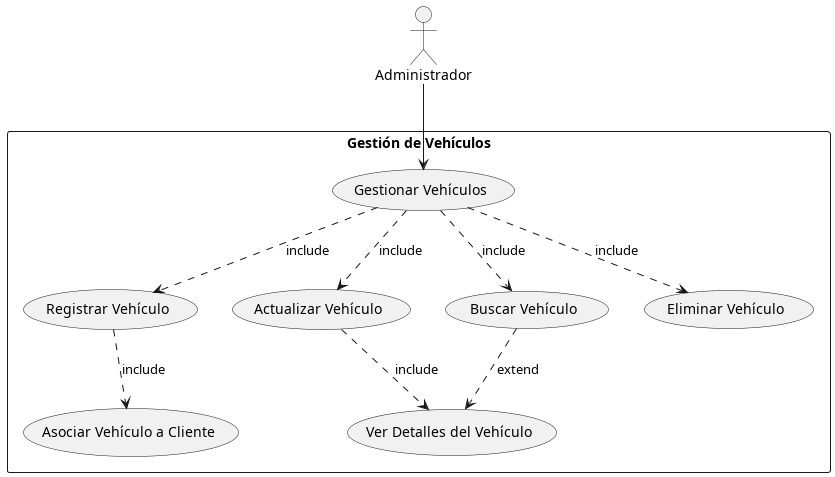
\includegraphics[width=12cm, height=7cm]{imagenes/cap4/casosUso/GestionVehiculos.png}
		\label{fig:Caso2}
	\end{figure}    
	
	\item Gestión de Servicios: Este paquete se dedica a las funcionalidades relacionadas con la gestión de servicios ofrecidos por el taller, incluyendo el registro, actualización, búsqueda y eliminación de servicios.
	\begin{itemize}
		\item \textbf{Gestionar Servicios:} Permite al administrador acceder a todas las funcionalidades relacionadas con los servicios.
		\item \textbf{Registrar Servicio:} Permite al administrador registrar un nuevo servicio en el sistema.
		\item \textbf{Actualizar Servicio:} Permite al administrador actualizar la información de un servicio existente.
		\item \textbf{Buscar Servicio:} Permite al administrador buscar servicios en la base de datos según ciertos criterios.
		\item \textbf{Eliminar Servicio:} Permite al administrador eliminar un servicio del sistema.
		\item \textbf{Asignar Precio:} Permite al administrador establecer o modificar el precio de un servicio.
		\item \textbf{Categorizar Servicio:} Permite al administrador asignar una categoría a un servicio para su mejor organización.
	\end{itemize}
	\begin{figure}[H]
		\centering
		\caption{Gestión de Servicios}
		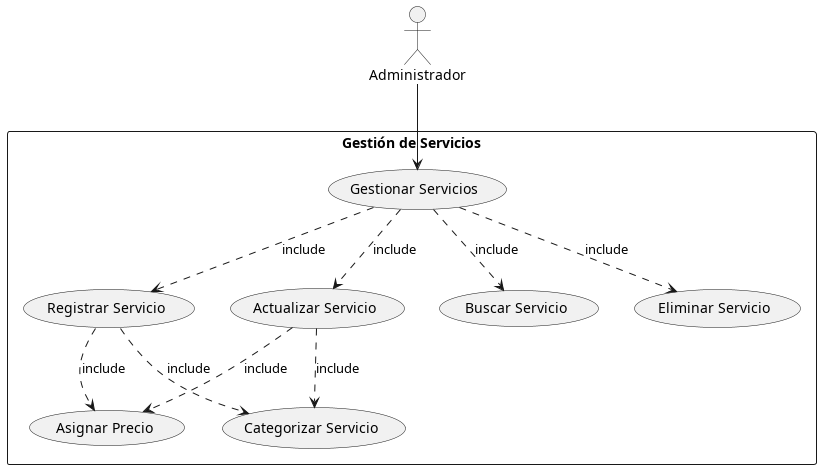
\includegraphics[width=12cm, height=8cm]{imagenes/cap4/casosUso/GestionServicios.png}
		\label{fig:Caso3}
	\end{figure}
	
	\item Gestión de Trabajos:
	Este paquete se encarga de la gestión de las órdenes de trabajo en el taller, abarcando desde el registro de nuevas órdenes hasta su seguimiento y actualización.
	\begin{itemize}
		\item \textbf{Gestionar Trabajos:} Permite al administrador acceder a todas las funcionalidades relacionadas con los trabajos y órdenes.
		\item \textbf{Registrar Orden:} Permite al administrador registrar una nueva orden de trabajo en el sistema.
		\item \textbf{Actualizar Orden:} Permite al administrador actualizar la información de una orden de trabajo existente.
		\item \textbf{Buscar Orden:} Permite al administrador buscar órdenes de trabajo en la base de datos según ciertos criterios.
		\item \textbf{Seguimiento de Orden:} Permite al administrador realizar el seguimiento del estado de una orden de trabajo.
		\item \textbf{Asignar Trabajo a Técnico:} Permite al administrador asignar una orden de trabajo a un técnico específico.
		\item \textbf{Cerrar Orden:} Permite al administrador finalizar una orden de trabajo una vez completada.
	\end{itemize}
	\begin{figure}[H]
		\centering
		\caption{Gestión de Trabajos}
		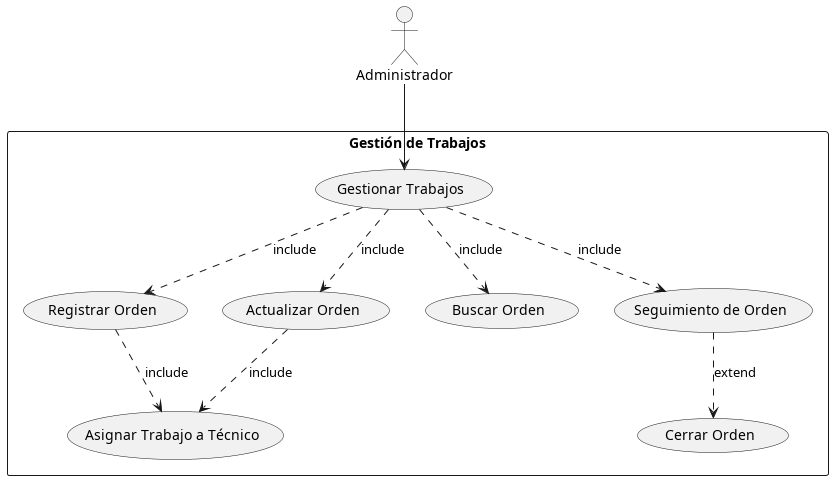
\includegraphics[width=12cm, height=10cm]{imagenes/cap4/casosUso/GestionTrabajos.png}
		\label{fig:Caso4}
	\end{figure}
	
	\item Gestión de Técnicos:
	Este paquete gestiona la información relacionada con los técnicos del taller, incluyendo el registro, actualización, búsqueda y eliminación de técnicos.
	\begin{itemize}
		\item \textbf{Gestionar Técnicos:} Permite al administrador acceder a todas las funcionalidades relacionadas con los técnicos.
		\item \textbf{Registrar Técnico:} Permite al administrador registrar un nuevo técnico en el sistema.
		\item \textbf{Actualizar Técnico:} Permite al administrador actualizar la información de un técnico existente en el sistema.
		\item \textbf{Buscar Técnico:} Permite al administrador buscar técnicos en la base de datos según ciertos criterios.
		\item \textbf{Eliminar Técnico:} Permite al administrador eliminar un técnico del sistema.
		\item \textbf{Ver Detalles del Técnico:} Permite al administrador obtener detalles específicos de un técnico registrado en el sistema.
		\item \textbf{Asignar Especialidad:} Permite al administrador asignar o modificar la especialidad de un técnico.
	\end{itemize}  
	\begin{figure}[H]
		\centering
		\caption{Gestión de Técnicos}
		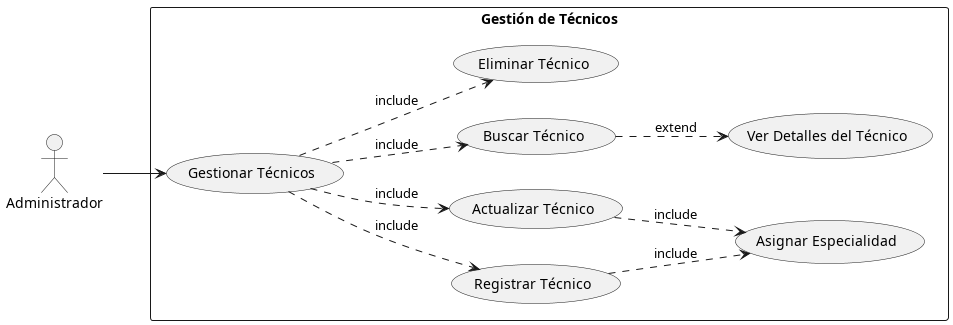
\includegraphics[width=12cm, height=8cm]{imagenes/cap4/casosUso/GestionTecnicos.png}
		\label{fig:Caso5}
	\end{figure}   
	
	\item Facturación:
	Este paquete maneja todas las funcionalidades relacionadas con la facturación de los servicios proporcionados, incluyendo el registro de costos, la generación de facturas y la gestión de los tipos de pago.
	\begin{itemize}
		\item \textbf{Gestionar Facturación:} Permite al administrador acceder a todas las funcionalidades relacionadas con la facturación.
		\item \textbf{Registrar Costos:} Permite al administrador registrar los costos asociados a los servicios realizados.
		\item \textbf{Generar Factura:} Permite al administrador generar una factura para los servicios prestados.
		\item \textbf{Procesar Pago:} Permite al administrador procesar el pago de una factura.
		\item \textbf{Pago con Tarjeta:} Permite al administrador gestionar pagos realizados con tarjeta.
		\item \textbf{Pago en Efectivo:} Permite al administrador gestionar pagos realizados en efectivo.
		\item \textbf{Anular Factura:} Permite al administrador anular una factura en caso de ser necesario.
	\end{itemize}
	\begin{figure}[H]
		\centering
		\caption{Facturación}
		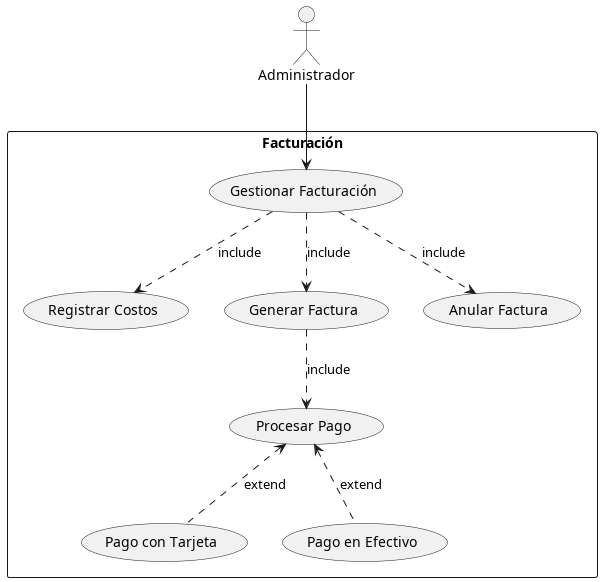
\includegraphics[width=12cm, height=9cm]{imagenes/cap4/casosUso/Facturacion.png}
		\label{fig:Caso6}
	\end{figure}      
	
	\item Reportes y Estadísticas:
	Este paquete se enfoca en la generación de reportes y la recopilación de estadísticas sobre los servicios proporcionados por el taller.
	\begin{itemize}
		\item \textbf{Gestionar Reportes:} Permite al administrador acceder a todas las funcionalidades relacionadas con reportes y estadísticas.
		\item \textbf{Generar Reporte de Ventas:} Permite al administrador generar un reporte detallado de las ventas realizadas.
		\item \textbf{Generar Reporte de Servicios:} Permite al administrador generar un reporte sobre los servicios prestados.
		\item \textbf{Ver Estadísticas:} Permite al administrador visualizar estadísticas generales sobre el rendimiento del taller.
		\item \textbf{Exportar Reportes:} Permite al administrador exportar los reportes generados en diferentes formatos.
		\item \textbf{Personalizar Reporte:} Permite al administrador ajustar los parámetros de los reportes según sus necesidades.
	\end{itemize}  
	\begin{figure}[H]
		\centering
		\caption{Reportes y Estadísticas}
		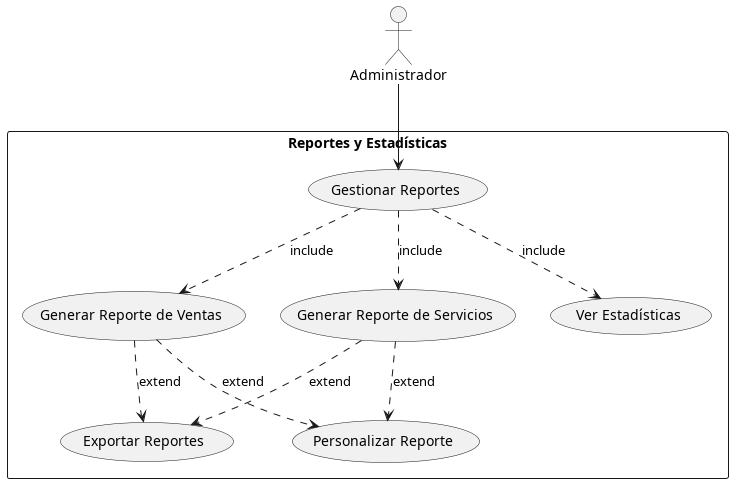
\includegraphics[width=12cm, height=8cm]{imagenes/cap4/casosUso/ReportesEstadisticas.png}
		\label{fig:Caso7}
	\end{figure}     
\end{enumerate}


\subsubsection*{4.2.3 Diagrama de clases}
%El diagrama de clases  en un representación visual de la estructura estática del sistema, muestra las clases, sus atributos y la forma en la que interactúan entre ellas. Este diagrama es útil para comprender la organización de los datos y las entidades del sistema. cada clase representa un conjunto de objetos con características similares, como usuario, clientes, vehículos, servicios, entre otros. Este diagrama forma parte del diseño para la implementación del sistema, permitiendo una mejor comprensión de su funcionamiento. Se puede ver en la pagina \pageref{fig:Dclases}

El diagrama de clases es una representación visual de la estructura estática del sistema, mostrando las clases, sus atributos y las relaciones entre ellas. Este diagrama es esencial para comprender la organización de los datos y las entidades que forman parte del sistema. Cada clase representa un conjunto de objetos con características similares, como usuarios, clientes, vehículos, servicios, entre otros. El diagrama de clases es una herramienta crucial en el diseño del sistema, ya que proporciona una visión detallada de la estructura del mismo, facilitando su implementación y asegurando una coherencia en la representación de los datos.

\subsubsection*{Descripción General}
\begin{enumerate}
    \item Cliente: Representa a los clientes, incluyendo su información de contacto y tipo de pago. Un cliente puede tener múltiples vehículos asociados.
    \item Vehículo: Registra los vehículos, con detalles como marca y modelo. Cada vehículo está vinculado a un cliente y puede tener múltiples órdenes de trabajo.
    \item Técnico: Describe a los técnicos del taller, con su especialidad y estado laboral. Cada técnico puede estar asignado a varias órdenes de trabajo.
    \item Servicios: Define los servicios que ofrece el taller, incluyendo el costo y la duración estimada. Los servicios son utilizados en las órdenes de trabajo.
    \item OrdenTrabajo: Gestiona las órdenes de trabajo para los vehículos, incluyendo los servicios realizados y el técnico asignado. Se registra la fecha de ingreso y salida del vehículo y el estado de la orden.
    \item Factura: Genera facturas vinculadas a un cliente, un vehículo y una orden de trabajo específica.
\end{enumerate}

\subsubsection*{Relaciones Clave}
\begin{itemize}
    \item Cliente-Vehículo: Un cliente puede poseer múltiples vehículos.
    \item Vehículo-OrdenTrabajo: Un vehículo puede tener varias órdenes de trabajo.
    \item OrdenTrabajo-Servicios: Una orden de trabajo puede incluir varios servicios.
    \item OrdenTrabajo-Técnico: Cada orden es atendida por un técnico específico.
    \item Factura: Relaciona un cliente, vehículo y orden de trabajo con una factura.    
\end{itemize}

%Diagrama de clases 
\begin{landscape}
    \begin{figure}
        \caption{Diagrama de clases}
        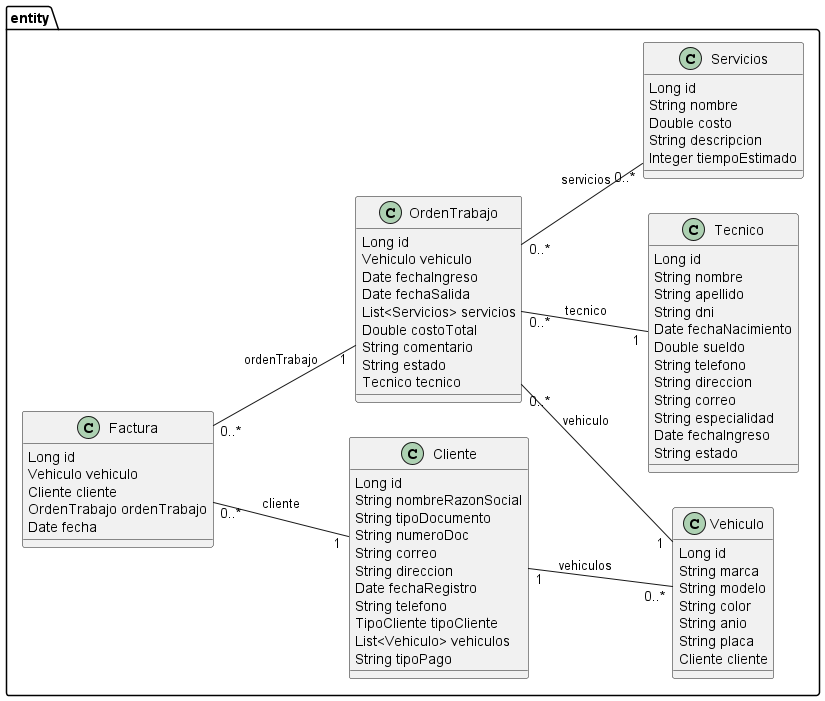
\includegraphics[width=22cm, height=16cm]{imagenes/cap4/ClaseInfoEntidad.png}
        \label{fig:Dclases}
    \end{figure}
\end{landscape}


\subsubsection*{4.2.4 Diagrama de Implementación}
Este diagrama es una representación visual de como se despliegan físicamente los componentes del sistema, incluyendo hardware y software, y cómo se comunican entre sí. Aquí se muestran los nodos físicos y las conexiones entre ellos, lo que ayuda a comprender la distribución de los diferentes elementos del sistema en el entorno de implementación. Es útil al planificar la infraestructura necesaria y asegurar una correcta implementación del sistema.

%\begin{landscape}
    \begin{figure}[H]
    \centering
    \caption[Diagrama de Implementación]{Diagrama de Implementación}
    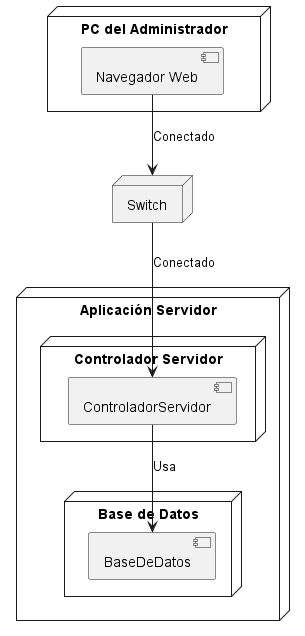
\includegraphics[width=8cm, height=15cm]{imagenes/cap4/diagramaImplementacion.png}
    \label{fig:DIMplementacion}
    \end{figure}
%\end{landscape}


\subsection{4.3 Recursos técnicos para implementar la mejora propuesta}
En esta sección, se detallan los recursos técnicos necesarios para llevar a cabo la implementación de la mejora propuesta. Se presentan los equipos, materiales, recursos humanos y documentación requeridos para el desarrollo y puesta en marcha del sistema. Cada tabla proporciona información sobre el tipo y cantidad de recursos necesarios, lo que permitirá una planificación más precisa y eficiente de los recursos disponibles para el proyecto. Esta fase es fundamental para asegurar que se cuenta con los medios adecuados para llevar a cabo la mejora de manera efectiva.

\begin{table}[H]
\centering
\caption{Equipos}
\label{tab:Equipos}
\begin{tblr}{
  cells = {c},
  row{1} = {ChetwodeBlue},
  rowsep = 3pt,
  hlines,
  vlines,
}
\textbf{Equipos} & \textbf{ Detalles}\\
Computadora & 1\\
Internet & 1
\end{tblr}
\end{table}

%\subsubsection*{Materiales}
\begin{table}[H]
\centering
\caption{Materiales}
\label{tab:Equipos}
\begin{tblr}{
  cells = {c},
  row{1} = {ChetwodeBlue},
  rowsep = 3pt,
  hlines,
  vlines,
}
\textbf{Software} & \textbf{ Detalles}\\
Lenguajes de Programación & 3\\
Base de datos & 1\\
Software de desarrollo & 1\\
Software de diseño & 1
\end{tblr}
\end{table}

%\subsubsection*{Recursos Humanos}
\begin{table}[H]
\centering
\caption{Recursos Humanos}
\label{tab:Equipos}
\begin{tblr}{
  cells = {c},
  row{1} = {ChetwodeBlue},
  rowsep = 3pt,
  hlines,
  vlines,
}
\textbf{Recursos Humanos} & \textbf{ Detalles}\\
Analista de Sistemas & 32 horas\\
Arquitecto de Software & 16 horas\\
Diseñador UX/UI & 32 horas\\
Desarrollador Front-End & 40 horas\\
Desarrollador Back-End & 64 horas\\
Tester & 24 horas
\end{tblr}
\end{table}



%\subsubsection*{Documentación}
\begin{table}[H]
\centering
\caption{Documentación}
\label{tab:Equipos}
\begin{tblr}{
  cells = {c},
  row{1} = {ChetwodeBlue},
  rowsep = 3pt,
  hlines,
  vlines,
}
\textbf{Documentación} & \textbf{ Detalles}\\
Lista de Requerimientos & 1\\
Documentación del Proyecto & 1
\end{tblr}
\end{table}


\subsection{4.4 Diagrama del proceso, mapa del flujo de valor y/o diagrama de operación de la situación mejorada}
En esta sección se presentara el diagrama de análisis de proceso mejorados, este diagrama reflejara los procesos mejorados y optimizados, considerando que el sistema de mejora ha sido implementado con éxito. Además, se destacarán los beneficios obtenidos a partir de estas mejoras, lo que permitirá visualizar claramente el impacto positivo en la eficiencia de los servicios ofrecidos.\\
En el diagrama 16 se puede ver la diferencia entre los tiempos de atención antes y después de la implementación de la mejora, ahorrando a la empresa 18 minutos durante cada servicio ofrecido.

\begin{figure}[H]
    \caption{Diagrama de Análisis de Proceso Mejorado}
    \begin{tabular}{c}
        %\includesvg[width=17cm, height=19cm]{imagenes/cap4/DAPmejorado.drawio.svg} \\
        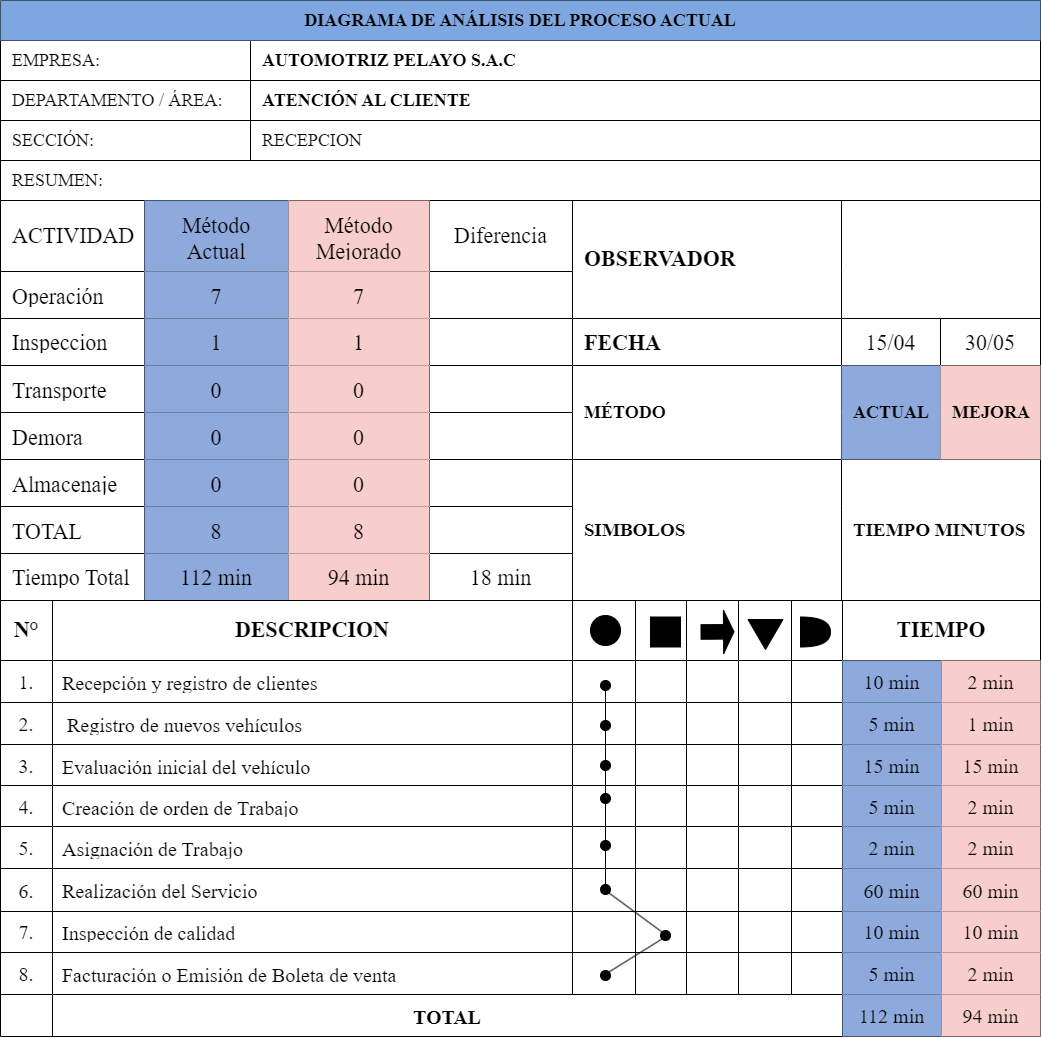
\includegraphics[width=16cm, height=18cm]{imagenes/cap4/DAPmejoradov2.drawio.png}
    \end{tabular}
    \label{fig:DAPMejorado}
\end{figure}


\subsection{4.5 Cronograma de ejecución de la mejora}
En esta sección se detalla el cronograma de ejecución de la mejora propuesta, donde se establece el orden en que se desarrollarán las actividades necesarias para llevar a cabo la implementación del proyecto de mejora. Cada actividad tiene asignado un responsable específico, como se muestra en la tabla 10. Este cronograma proporciona una visión general del tiempo requerido para cada tarea. Además, sirve como herramienta para detectar posibles retrasos en el cumplimiento de los plazos y actuar de inmediato.

\begin{table}[H]
\centering
\caption{Cronograma de ejecución de la mejora}
\label{tab:Cronograma}
\begin{tblr}{
  row{1} = {ChetwodeBlue},
  column{1} = {7cm},
  cell{1}{1} = {c},
  cell{2}{2} = {blue,c},
  cell{3}{3} = {blue,c},
  cell{4}{4} = {blue,c},
  cell{4}{5} = {c},
  cell{5}{5} = {blue,c},
  cell{5}{6} = {blue,c},
  cell{6}{6} = {blue},
  cell{6}{7} = {blue,c},
  cell{6}{8} = {c},
  cell{7}{7} = {blue},
  cell{7}{8} = {blue,c},
  cell{7}{9} = {c},
  cell{8}{8} = {blue},
  cell{8}{10} = {c},
  cell{9}{9} = {blue},
  cell{9}{10} = {blue},
  cell{9}{11} = {c},
  cell{10}{11} = {blue,c},
  hlines,
  vlines,
}
\textbf{Tiempo de Ejecución} & \textbf{S1} & \textbf{S2} & \textbf{S3} & \textbf{S4} & \textbf{S5} & \textbf{S6} & \textbf{S7} & \textbf{S8} & \textbf{S9} & \textbf{S10}\\
Listar
  requisitos del sistema &  &  &  &  &  &  &  &  &  & \\
Análisis
  de requisitos &  &  &  &  &  &  &  &  &  & \\
Diseño
  de la interfaz &  &  &  &  &  &  &  &  &  & \\
Desarrollo
  de la interfaz &  &  &  &  &  &  &  &  &  & \\
Diseño
  de la arquitectura Backend &  &  &  &  &  &  &  &  &  & \\
Implementación
  del Back-End &  &  &  &  &  &  &  &  &  & \\
Unión
  del Front-End y Back-End &  &  &  &  &  &  &  &  &  & \\
Pruebas
  de funcionamiento &  &  &  &  &  &  &  &  &  & \\
Implementación del sistema en entorno de
  producción &  &  &  &  &  &  &  &  &  & 
\end{tblr}
\end{table}


\subsection{4.6 Aspectos limitantes para la implementación de la mejora}
En esta sección se abordara las limitaciones o dificultades que surgen durante la implementación de la acción de mejora pueden ser un factor clave a tomar en cuenta, puesto que pueden llegar a determinar la consecución, o no del proyecto. Algunas de las dificultades que surgieron la implementación fueron las siguientes:
\begin{enumerate}
    \item Recursos financieros limitados: La disponibilidad de fondos puede ser un factor restrictivo, ya que algunas mejoras pueden requerir una inversión significativa en tecnología, capacitación de personal o infraestructura.
    \item Resistencia al cambio: El cambio puede enfrentar resistencia por parte de los empleados que están acostumbrados a los procesos antiguos o temen la pérdida de control sobre su trabajo.
    \item Factor de Tiempo: Algunos plazos ajustados pueden dificultar el cumplimiento adecuado de todas las etapas del proyecto. Esto puede llevar a la necesidad de priorizar ciertas actividades sobre otras o comprometer la calidad del trabajo realizado.
    \item Limitaciones técnicas: Pueden surgir desafíos técnicos durante la implementación, como problemas de compatibilidad entre diferentes sistemas. Esta complejidad técnica puede ralentizar el progreso del proyecto y requerir soluciones rápidas para superar los obstáculos.
\end{enumerate}
\begin{table}[H]
\centering
\caption{Diagrama de Limitaciones}
\label{tab:Equipos}
\begin{tblr}{
  column{1} = {wd=1cm},
  column{2} = {wd=5.4cm},
  column{3} = {wd=8.9cm},
  row{1} = {ChetwodeBlue,c},
  cell{2}{1} = {c},
  cell{3}{1} = {c},
  cell{4}{1} = {c},
  cell{5}{1} = {c},
  hlines,
  vlines,
}
\textbf{Ítem} & \textbf{Aspecto Observado} & \textbf{Indicador}\\
01 & Recursos financieros limitados & Disponibilidad limitada de fondos para inversión\\
02 & Resistencia al cambio & Actitudes negativas hacia la implementación de mejoras\\
03 & Factor de tiempo & Plazos ajustados para cumplir con todas las etapas del proyecto\\
04 & Limitaciones técnicas & Problemas de compatibilidad entre sistemas o tecnologías
\end{tblr}
\end{table}








%Diagrama de Ganttt
%\begin{landscape}
%    \hspace{3cm}
%    \begin{table}[h]
%    \captionsetup{labelformat=empty}
%    \caption[Diagrama de Gantt]{\textbf{Diagrama de Gantt realizado en GanntProyect}}
%    \begin{tabular}{c}
%        \includegraphics[width=22cm, height=10cm]{imagenes/cap4/DiagramaGant1.jpg}
%    \end{tabular}    
%    \label{fig:DiagramaGant}
%\end{table}
%\end{landscape}


%cuidar el pie de pagina.. 
%referencianr por el numero de diagrama o grafico
%la imagen del los casos de uso deben ser del mismo tamaño